\documentclass{article}

\usepackage{fancyhdr}
\usepackage{extramarks}
\usepackage{amsmath}
\usepackage{amsthm}
\usepackage{amsfonts}
\usepackage{tikz}
\usepackage[plain]{algorithm}
\usepackage{algpseudocode}
\usepackage{xcolor}
\usepackage{amssymb}
\usepackage{todonotes}
\usepackage{mathtools}
\usepackage{cancel}
\usepackage{listings}
\usepackage{dirtytalk}
\usepackage{soul}
\usetikzlibrary{decorations.pathreplacing}
\usepackage{hyperref}
\usepackage{parcolumns}
\usepackage{tabularx}
\usepackage{caption}
\usepackage{lastpage}
\usepackage{color}
\usepackage[inline]{enumitem}


\definecolor{mygreen}{rgb}{0,0.6,0}
\definecolor{mygray}{rgb}{0.5,0.5,0.5}
\definecolor{mymauve}{rgb}{0.58,0,0.82}

\lstset{
  backgroundcolor=\color{white},   % choose the background color; you must add \usepackage{color} or \usepackage{xcolor}; should come as last argument
  basicstyle=\footnotesize,        % the size of the fonts that are used for the code
  breakatwhitespace=false,         % sets if automatic breaks should only happen at whitespace
  breaklines=true,                 % sets automatic line breaking
  captionpos=b,                    % sets the caption-position to bottom
  commentstyle=\color{mygreen},    % comment style
  deletekeywords={...},            % if you want to delete keywords from the given language
  escapeinside={\%*}{*)},          % if you want to add LaTeX within your code
  extendedchars=true,              % lets you use non-ASCII characters; for 8-bits encodings only, does not work with UTF-8
  frame=single,	                   % adds a frame around the code
  keepspaces=true,                 % keeps spaces in text, useful for keeping indentation of code (possibly needs columns=flexible)
  keywordstyle=\color{orange!90!black},       % keyword style
  language=Python,                 % the language of the code
  morekeywords={*,...},            % if you want to add more keywords to the set
  numbers=left,                    % where to put the line-numbers; possible values are (none, left, right)
  numbersep=5pt,                   % how far the line-numbers are from the code
  numberstyle=\tiny\color{mygray}, % the style that is used for the line-numbers
  rulecolor=\color{black},         % if not set, the frame-color may be changed on line-breaks within not-black text (e.g. comments (green here))
  showspaces=false,                % show spaces everywhere adding particular underscores; it overrides 'showstringspaces'
  showstringspaces=false,          % underline spaces within strings only
  showtabs=false,                  % show tabs within strings adding particular underscores
  stepnumber=1,                    % the step between two line-numbers. If it's 1, each line will be numbered
  stringstyle=\color{yellow!60!orange!80!black},     % string literal style
  tabsize=2,	                   % sets default tabsize to 2 spaces
  title=\lstname,                   % show the filename of files included with \lstinputlisting; also try caption instead of title
  keywords=[3]{self},
  keywordstyle=[3]{\color{orange!50!gray}},
  keywords=[4]{__init__, __lt__},
  keywordstyle=[4]{\color{orange!50!gray}},
  moredelim=**[is][\color{orange!90!black}]{@}{@}
}


\usetikzlibrary{automata,positioning}

%
% Basic Document Settings
%

\topmargin=-0.45in
\evensidemargin=0in
\oddsidemargin=0in
\textwidth=6.5in
\textheight=9.0in
\headsep=0.25in

\linespread{1.1}

\pagestyle{fancy}
\lhead{\hmwkAuthorName}
\chead{\hmwkClass\ (\hmwkClassInstructor): \hmwkTitle}
\rhead{\firstxmark}
\lfoot{\lastxmark}
\cfoot{Page \thepage\ of \pageref{LastPage}}

\renewcommand\headrulewidth{0.4pt}
\renewcommand\footrulewidth{0.4pt}

%
% Create Exercise Sections
%

\newcommand{\enterExerciseHeader}[1]{
    \nobreak\extramarks{}{Exercise \arabic{#1} continued on next page\ldots}\nobreak{}
    \nobreak\extramarks{Exercise \arabic{#1} (continued)}{Exercise \arabic{#1} continued on next page\ldots}\nobreak{}
}

\newcommand{\exitExerciseHeader}[1]{
    \nobreak\extramarks{Exercise \arabic{#1} (continued)}{Exercise \arabic{#1} continued on next page\ldots}\nobreak{}
    \stepcounter{#1}
    \nobreak\extramarks{Exercise \arabic{#1}}{}\nobreak{}
}

\newcount\colveccount
\newcommand*\colvec[1]{
        \global\colveccount#1
        \begin{pmatrix}
        \colvecnext
}
\def\colvecnext#1{
        #1
        \global\advance\colveccount-1
        \ifnum\colveccount>0
                \\
                \expandafter\colvecnext
        \else
                \end{pmatrix}
        \fi
}

\setcounter{secnumdepth}{0}
\newcounter{partCounter}
\newcounter{homeworkExerciseCounter}
\setcounter{homeworkExerciseCounter}{1}
\nobreak\extramarks{Exercise \arabic{homeworkExerciseCounter}}{}\nobreak{}

%
% Homework Exercise Environment
%
% This environment takes an optional argument. When given, it will adjust the
% Exercise counter. This is useful for when the Exercises given for your
% assignment aren't sequential. See the last 3 Exercises of this template for an
% example.
%
\newenvironment{homeworkExercise}[1][-1]{
    \ifnum#1>0
        \setcounter{homeworkExerciseCounter}{#1}
    \fi
    \section{Exercise \arabic{homeworkExerciseCounter}}
    \setcounter{partCounter}{1}
    \enterExerciseHeader{homeworkExerciseCounter}
}{
    \exitExerciseHeader{homeworkExerciseCounter}
}

%
% Homework Details
%   - Title
%   - Due date
%   - Class
%   - Section/Time
%   - Instructor
%   - Author
%

\newcommand{\hmwkTitle}{Assignment 4}
\newcommand{\hmwkDueDate}{May 21, 2018}
\newcommand{\hmwkClass}{Algorithms}
\newcommand{\hmwkClassTime}{Spring Semester}
\newcommand{\hmwkClassInstructor}{Prof. Antonio Carzaniga}
\newcommand{\hmwkAuthorName}{\textbf{A. Romanelli}}

%
% Title Page
%

\title{
    \vspace{2in}
    \textmd{\textbf{\hmwkClass:\ \hmwkTitle}}\\
    \normalsize\vspace{0.1in}\small{Due\ on\ \hmwkDueDate\ at 20:00}\\
    \vspace{0.1in}\large{\textit{\hmwkClassInstructor}}
    \vspace{3in}
}

\author{\hmwkAuthorName}
\date{}

\renewcommand{\part}[1]{\textbf{\large Part \Alph{partCounter}}\stepcounter{partCounter}\\}


%
% Various Helper Commands
%

% Useful for algorithms
\newcommand{\alg}[1]{\textsc{\bfseries \footnotesize #1}}

% For derivatives
\newcommand{\deriv}[1]{\frac{\mathrm{d}}{\mathrm{d}x} (#1)}

% For partial derivatives
\newcommand{\pderiv}[2]{\frac{\partial}{\partial #1} (#2)}

% Integral dx
\newcommand{\dx}{\mathrm{d}x}

% Alias for the Solution section header
\newcommand{\solution}{\textbf{\large Solution}}

% Probability commands: Expectation, Variance, Covariance, Bias
\newcommand{\E}{\mathrm{E}}
\newcommand{\Var}{\mathrm{Var}}
\newcommand{\Cov}{\mathrm{Cov}}
\newcommand{\Bias}{\mathrm{Bias}}

\begin{document}

\maketitle

\pagebreak

\begin{homeworkExercise}
We are considering a graph $G$ and we want to write a Python program that computes and prints the articulation points of $G$. We should point out that an articulation point is any given point of the graph $G$, such that if it is removed, the graph becomes disconnected. \\
\begin{figure}[h]
	\centering
	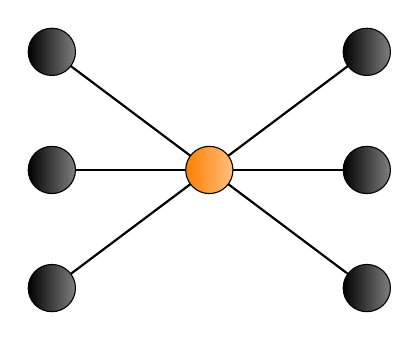
\begin{tikzpicture}
		\draw[thick] (-2,0) -- (0,0) -- (2,0);
		\draw[thick] (-2,-1.5) -- (0,0) -- (2,1.5);
		\draw[thick] (2,-1.5) -- (0,0) -- (-2,1.5);
		\draw[left color=orange, right color=orange!50!white] (0,0) circle (3mm);
		\draw[left color=black, right color=black!50!white] (2,0) circle (3mm);
		\draw[left color=black, right color=black!50!white] (-2,0) circle (3mm);
		\draw[left color=black, right color=black!50!white] (2,1.5) circle (3mm);
		\draw[left color=black, right color=black!50!white] (-2,1.5) circle (3mm);
		\draw[left color=black, right color=black!50!white] (2,-1.5) circle (3mm);
		\draw[left color=black, right color=black!50!white] (-2,-1.5) circle (3mm);
	\end{tikzpicture}
	\caption{Representation of an \textcolor{orange!90!black}{articulation point} of a given $G$}
\end{figure}\\
I decided to implement my graph in Python with an adjacency list: this means that my \verb|Graph| structure is going to contain the following general properties: 
\begin{itemize}
	\item The number of vertices: \verb|self.size|;
	\item The adjacent vertices to every vertex: \verb|self.edges[[]]|. \\
	(Each vertex is assigned a list of other vertices, which define the edges of the graph);
	\item A global counter, which is going to keep track of \say{time}: \verb|self.globalTime|.
\end{itemize}
Now, my idea is to \say{map} every vertex to more specific properties:
\begin{figure}[h]
	\centering
	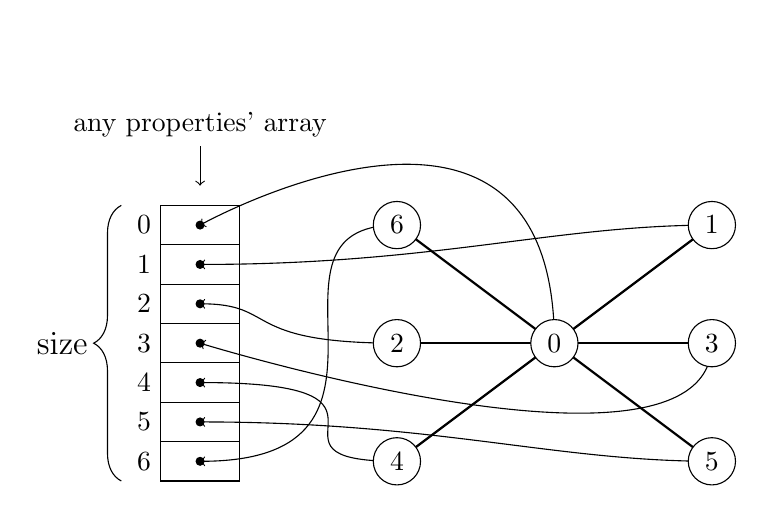
\begin{tikzpicture}
		\draw[thick] (-2,0) -- (0,0) -- (2,0);
		\draw[thick] (-2,-1.5) -- (0,0) -- (2,1.5);
		\draw[thick] (2,-1.5) -- (0,0) -- (-2,1.5);
		
		\draw[->] (0,0) .. controls +(up:4cm) and +(right:0cm) .. (-4.5,1.5);
		\draw[->] (2,1.5) .. controls +(left:2cm) and +(right:3cm) .. (-4.5,1);
		\draw[->] (-2,0) .. controls +(left:2cm) and +(right:1cm) .. (-4.5,0.5);
		\draw[->] (2,0) .. controls +(down:2cm) and +(down:0cm) .. (-4.5,0);
		\draw[->] (-2,-1.5) .. controls +(left:2cm) and +(right:3cm) .. (-4.5,-0.5);
		\draw[->] (2,-1.5) .. controls +(left:2cm) and +(right:3cm) .. (-4.5,-1);
		\draw[->] (-2,1.5) .. controls +(left:2cm) and +(right:3cm) .. (-4.5,-1.5);
		
		\draw[fill=white] (0,0) circle (3mm)
			node {0};
		\draw[fill=white] (2,0) circle (3mm)
			node {3};
		\draw[fill=white] (-2,0) circle (3mm)
			node {2};
		\draw[fill=white] (2,1.5) circle (3mm)
			node {1};
		\draw[fill=white] (-2,1.5) circle (3mm)
			node {6};
		\draw[fill=white] (2,-1.5) circle (3mm)
			node {5};
		\draw[fill=white] (-2,-1.5) circle (3mm)
			node {4};
			
			
		\foreach \i in {0,...,6} {
			
			\draw (-5,1.75) rectangle (-4,1.25-\i*0.5)
			node[anchor=east] at (-5,1.5-\i*0.5) {\i};
			\draw[fill=black] (-4.5,1.5-\i*0.5) circle (0.5mm);
		}
		
		\draw[<-] (-4.5, 2) -- (-4.5, 2.5)
			node[anchor=south] {any properties' array};
		
		\draw [decorate,decoration={brace,amplitude=10pt,mirror,raise=0pt},yshift=0pt]
(-5.5, 1.75) -- (-5.5, -1.75) node [black,midway,xshift=-0.75cm,yshift=0] {\large size};
		
	\end{tikzpicture}
\end{figure} \\
The result is a one-to-many correspondence between a node and its properties, which are stored in array within the graph. For this exercise I implemented the following vertex properties: \\ \\
\begin{minipage}{0.5\textwidth}
	\begin{itemize}
		\item Adjacent vertices;
		\item Time of first visit;
		\item Fastest visit time;
	\end{itemize}
\end{minipage}
\begin{minipage}{0.5\textwidth}
	\begin{itemize}
		\item Previous vertex;
		\item Flag whether the vertex is an articulation point;
		\item A colour to flag whether we visited the vertex already.
	\end{itemize}
\end{minipage}
\newpage
\begin{figure}
	\centering
	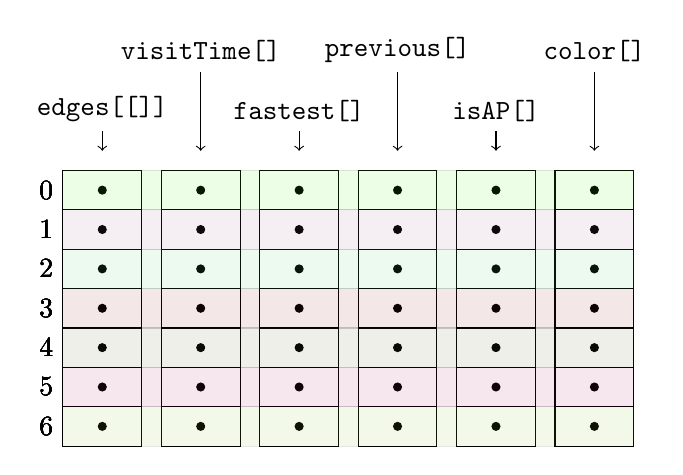
\begin{tikzpicture}
			
		\foreach \j in {0,...,5} {
			\foreach \i in {0,...,6} {
				\draw (-1+\j*1.25,1.75) rectangle (0+\j*1.25,1.25-\i*0.5)
					node[anchor=east] at (-1,1.5-\i*0.5) {\i};
				\draw[fill=black] (-0.5+\j*1.25,1.5-\i*0.5) circle (0.5mm);
			}
		}
		\draw[<-] (-0.5, 2) -- (-0.5, 2.25)
			node[anchor=south] {\verb|edges[[]]|};
			
		\draw[<-] (0.75, 2) -- (0.75, 3)
			node[anchor=south] {\verb|visitTime[]|};	
			
		\draw[<-] (2, 2) -- (2, 2.25)
			node[anchor=south] {\verb|fastest[]|};		
			
		\draw[<-] (3.25, 2) -- (3.25, 3)
			node[anchor=south] {\verb|previous[]|};	
			
		\draw[<-] (4.5, 2) -- (4.5, 2.25)
			node[anchor=south] {\verb|isAP[]|};	
			
		\draw[<-] (5.75, 2) -- (5.75, 3)
			node[anchor=south] {\verb|color[]|};	
			
		\foreach \i in {0,...,6} {
			\edef\R{\pdfuniformdeviate 255}
			\edef\G{\pdfuniformdeviate 255}
			\edef\B{\pdfuniformdeviate 255}
			\xdefinecolor{MyColor}{RGB}{\R,\G,\B}
			\draw[fill=MyColor, opacity=0.1] (-1,1.75-\i*0.5) rectangle (6.25,1.25-\i*0.5); 
		}
	\end{tikzpicture}
	\caption{Each row in this column space represents the set of properties common to a given vertex.}
\end{figure}
From my illustrations it clearly follows that the properties of the vertices can be grouped up into arrays of length $|G|$, so that to access a property of a given vertex $v$ one can simply access \verb|property[v]|:\\	
\lstinputlisting[firstline=5, lastline=21, title=\ , firstnumber=1]{ex1.py}
\vspace{-0.5cm}
The only code here worth explaining might be the initialisation of \verb|self.edges|, which gave me a lot of problems initially, since I was creating it like so:
\begin{lstlisting}
	self.edges = [[]]*size
\end{lstlisting}
\vspace{-0.5cm}
But this would instantiate a multidimensional array having as element the same reference to another array, however this was only a Python's pettiness. \\ \\ 
The \verb|insertEdge(u,v)| method takes care of establishing a non-directed edge between two vertices. \\ \\

To find out the articulation points in the graph $G$, I'm going to use a \emph{Depth First Search algorithm}, because I want to find vertices with two possible specific properties. \\ \\
An articulation point is then a such point if it satisfies one of the following two conditions when contained in a \emph{Depth First Search tree}:\\ \\
\begin{minipage}{0.4\textwidth}
	\centering
	A node is at the root of the tree of the \emph{Depth First Search} and has two children.
\end{minipage}\hfill
\begin{minipage}{0.4\textwidth}
	A node is not at the root of the \emph{DFS} tree and it has a child which is the only connection to its adjacent nodes.
\end{minipage} \\ \\ \\
The first condition is evident by the fact that in a \emph{DFS}, if a vertex has more then two children it means that it already recursed all the way to the bottom and could not traverse between the two branches and thus the vertex at the root is an articulation point. \\ \\
We are going to implement this search recursively and in order to do that we will have our case to be when all the nodes of the graph are visited and we are going to use an helper function in order to recurse on the adjacent vertices when iterating on each one of them.

\lstinputlisting[firstline=43, lastline=57, title=\ , firstnumber=39]{ex1.py}
\vspace{-0.5cm}
For each vertex present in the graph that hasn't been visited yet we are going to check whether it is an articulation point. Once we have flagged all our articulation points, we are going again to iterate over all the vertices and print out the ones that were flagged.
\lstinputlisting[firstline=22, lastline=42, title=\ , firstnumber=17]{ex1.py}
\vspace{-0.5cm}
The first thing we do when we access a vertex is to make sure we flag it as a vertex that is currently being visited (colour \say{gray}), then we can log into its corresponding property key the time at which we discovered the vertex. Then we initialise the children counter to zero and make sure to step forward to global timer by one unit.
\newpage
Secondly, we will want to traverse to the adjacent vertices just like we would normally do with our \emph{DFS} tree, keeping count of the children and by properly flagging our vertices. Each adjacent vertex will also be recursively checked for the conditions of existence of an articulation point. 
\begin{figure}[h]
	\centering
	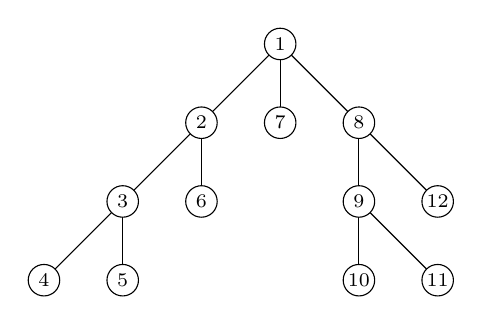
\begin{tikzpicture}
		\draw (-3,-3) -- (0,0) -- (2,-2);
		\draw (-2,-2) -- (-2,-3);
		\draw (-1,-1) -- (-1,-2);
		\draw (0,0) -- (0,-1);
		\draw (1,-1) -- (1,-3);
		\draw (1,-2) -- (2,-3);
		\draw[fill=white] (0,0) circle (2mm)
			node {\scriptsize 1};
		\draw[fill=white] (-1,-1) circle (2mm)
			node {\scriptsize 2};	
		\draw[fill=white] (-2,-2) circle (2mm)
			node {\scriptsize 3};	
		\draw[fill=white] (-3,-3) circle (2mm)
			node {\scriptsize 4};
		\draw[fill=white] (-2,-3) circle (2mm)
			node {\scriptsize 5};		
		\draw[fill=white] (-1,-2) circle (2mm)
			node {\scriptsize 6};		
		\draw[fill=white] (0,-1) circle (2mm)
			node {\scriptsize 7};	
		\draw[fill=white] (1,-1) circle (2mm)
			node {\scriptsize 8};			
		\draw[fill=white] (1,-2) circle (2mm)
			node {\scriptsize 9};
		\draw[fill=white] (1,-3) circle (2mm)
			node {\scriptsize 10};		
		\draw[fill=white] (2,-3) circle (2mm)
			node {\scriptsize 11};	
		\draw[fill=white] (2,-2) circle (2mm)
			node {\scriptsize 12};	
	\end{tikzpicture}
	\caption{Order in which the nodes of the \emph{DFS} tree are visited from node \textbf{1}, which corresponds to the \emph{visitTime} property.}
\end{figure}\\
Finally we check whether the two above-stated conditions actually verify and if that is the case we assign the key of the vertex with the appropriate boolean flag. I also had to log an additional property, namely \verb|fastest|, which is a property that keeps track of whether the node could have been accessed in a faster way than its initial \verb|visitTime|, it is always smaller or equal than the \verb|visitTime|. \\ \\
I'll show with an example the implementation of our second condition of existence given the following example:
\begin{figure}[h]
	\centering
	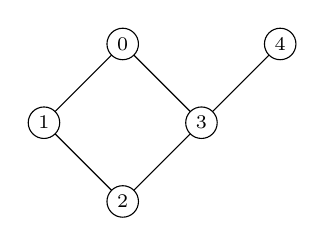
\begin{tikzpicture}
		\draw (0,0) -- (1,-1) -- (0,-2) -- (-1,-1) -- cycle;
		\draw (1,-1) -- (2,0);
		\draw[fill=white] (2,0) circle (2mm)
			node {\scriptsize 4};
		\draw[fill=white] (0,0) circle (2mm)
			node {\scriptsize 0};
		\draw[fill=white] (-1,-1) circle (2mm)
			node {\scriptsize 1};
		\draw[fill=white] (0,-2) circle (2mm)
			node {\scriptsize 2};
		\draw[fill=white] (1, -1) circle (2mm)
			node {\scriptsize 3};
	\end{tikzpicture}	
	\caption{The graph has only one articulation point being at node \textbf{3}.}
\end{figure} \\
Our first condition of existence in this case would not apply, since the node \textbf{3} is not at the root of our \emph{DFS}. The iteration in this case is going to look as follows: \\ \\
\begin{minipage}{0.5\linewidth}
	\centering
	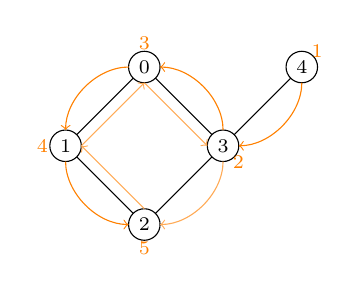
\begin{tikzpicture}
		\draw (0,0) -- (1,-1) -- (0,-2) -- (-1,-1) -- cycle;
		\draw (1,-1) -- (2,0);
		\draw[fill=white] (2,0) circle (2mm)
			node {\scriptsize 4};
		\node[anchor=south west] at (2,0) {\color{orange}\scriptsize 1};
		\draw[fill=white] (0,0) circle (2mm)
			node {\scriptsize 0};
		\node[anchor=south] at (0,0.1) {\color{orange}\scriptsize 3};
		\draw[fill=white] (-1,-1) circle (2mm)
			node {\scriptsize 1};
		\node[anchor=east] at (-1.1,-1) {\color{orange}\scriptsize 4};
		\draw[fill=white] (0,-2) circle (2mm)
			node {\scriptsize 2};
		\node[anchor=north] at (0,-2.1) {\color{orange}\scriptsize 5};
		\draw[fill=white] (1, -1) circle (2mm)
			node {\scriptsize 3};
		\node[anchor=north west] at (1,-1) {\color{orange}\scriptsize 2};
		\draw[->,color=orange]  (2,-0.2) .. controls +(down:0.4cm) and +(right:0.4cm) .. (1.2,-1);
		\draw[->, color=orange] (1,-0.8) .. controls +(up:0.4cm) and +(right:0.4cm) .. (0.2,0);
		\draw[->, color=orange] (-0.2,0) .. controls +(left:0.4cm) and +(up:0.4cm) .. (-1,-0.8);
		\draw[->, color=orange] (-1,-1.2) .. controls +(down:0.4cm) and +(left:0.4cm) .. (-0.2,-2);
		\draw[->, color=orange!66!white] (0,-1.8) -- (-0.8,-1);
		\draw[->, color=orange!66!white] (-0.8,-1) -- (0,-0.2);
		\draw[->, color=orange!66!white] (0,-0.2) -- (0.8,-1);
		\draw[->, color=orange!66!white] (1,-1.2) .. controls +(down:0.4cm) and +(right: 0.4cm) .. (0.2,-2);
	\end{tikzpicture}\\
	\captionof{figure}{Visit times of the nodes in the graph}
\end{minipage}
\begin{minipage}{0.5\linewidth}
	\centering	
	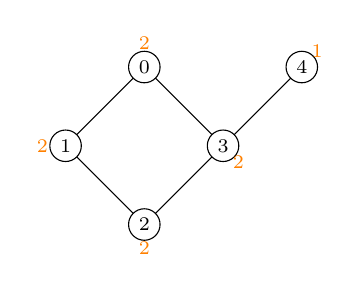
\begin{tikzpicture}
		\draw (0,0) -- (1,-1) -- (0,-2) -- (-1,-1) -- cycle;
		\draw (1,-1) -- (2,0);
		\draw[fill=white] (2,0) circle (2mm)
			node {\scriptsize 4};
		\node[anchor=south west] at (2,0) {\color{orange}\scriptsize 1};
		\draw[fill=white] (0,0) circle (2mm)
			node {\scriptsize 0};
		\node[anchor=south] at (0,0.1) {\color{orange}\scriptsize 2};
		\draw[fill=white] (-1,-1) circle (2mm)
			node {\scriptsize 1};
		\node[anchor=east] at (-1.1,-1) {\color{orange}\scriptsize 2};
		\draw[fill=white] (0,-2) circle (2mm)
			node {\scriptsize 2};
		\node[anchor=north] at (0,-2.1) {\color{orange}\scriptsize 2};
		\draw[fill=white] (1, -1) circle (2mm)
			node {\scriptsize 3};
		\node[anchor=north west] at (1,-1) {\color{orange}\scriptsize 2};
%		\draw[->,color=orange]  (2,-0.2) .. controls +(down:0.4cm) and +(right:0.4cm) .. (1.2,-1);
%		\draw[->, color=orange] (1,-0.8) .. controls +(up:0.4cm) and +(right:0.4cm) .. (0.2,0);
%		\draw[->, color=orange] (-0.2,0) .. controls +(left:0.4cm) and +(up:0.4cm) .. (-1,-0.8);
%		\draw[->, color=orange] (-1,-1.2) .. controls +(down:0.4cm) and +(left:0.4cm) .. (-0.2,-2);
%		\draw[->, color=orange!66!white] (0,-1.8) -- (-0.8,-1);
%		\draw[->, color=orange!66!white] (-0.8,-1) -- (0,-0.2);
%		\draw[->, color=orange!66!white] (0,-0.2) -- (0.8,-1);
%		\draw[->, color=orange!66!white] (1,-1.2) .. controls +(down:0.4cm) and +(right: 0.4cm) .. (0.2,-2);
	\end{tikzpicture}	
	\captionof{figure}{Fastest times of the nodes in the graph}
\end{minipage}\\ \\
If the following condition is true:
\begin{lstlisting}
	if self.previous[vertex] != None and self.fastest[adj] >= self.visitTime[vertex]
\end{lstlisting}
\vspace{-0.75cm}
It must mean that when iterating through the adjacent vertices, we somehow found a way to reconnect ourselves to our initial node or another node that was visited before the one we started from, and its fastest time was transmitted to all the nodes from the bottom of the recursion.

\subsection{Complexity Analysis}
Our complexity will be the same as a normal DFS tree which is \textemdash\ as we know from theory \textemdash\ in the order of $\mathcal{O}(n+m)$ with some additional book-keeping, modifying the arrays stored within the \verb|Graph| structure in constant time. Then we only iterate $2n$ times to compute the amounts of articulation points and to print all of them. Thus, our overall complexity will be $\mathcal{O}(n+m)$.
%Our target complexity is $\mathcal{O}(n+m)$. Our main function iterates through all the vertices of the graph and for each of those it runs \verb|checkVertex|. Within the \verb|checkVertex| function we will perform constant time operations and later iterate over any adjacent vertices that have not been visited yet. If they have not been visited, we'll run \verb|checkVertex| on them, which again takes constant time and recurses on its adjacent vertices, else we do something only if the adjacent vertex isn't the vertex from which we are coming from. \\ \\

\end{homeworkExercise}
\newpage
\begin{homeworkExercise}
	We are given a maze that is composed by $n \times m$ of equally sized cells, that are arranged in a grid and that can be four different types:
	\begin{center}
		\begin{itemize*}[label=\ ]
			\item 
			\begin{tikzpicture}[scale=0.25]
				\draw (0,0) -- (0,1) -- (1,1) -- (1,0) -- cycle;
			\end{tikzpicture} Empty \textemdash
			\item 
			
\begin{tikzpicture}[scale=0.25]
				\fill (0,0) -- (0,1) -- (1,1) -- (1,0) -- cycle;
			\end{tikzpicture}
			Blocked \textemdash
			\item 
			
\begin{tikzpicture}[scale=0.25]
				\filldraw[color=orange!75!white, draw=black] (0,0) -- (0,1) -- (1,1) -- (1,0) -- cycle;
			\end{tikzpicture}
			Start \textemdash
			\item 
			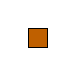
\begin{tikzpicture}[scale=0.25]
				\filldraw[color=orange!75!black, draw=black] (0,0) -- (0,1) -- (1,1) -- (1,0) -- cycle;
			\end{tikzpicture}
			Exit
		\end{itemize*}
	\end{center}
	Starting from the start block, our task is to find the exit, if we can find it, with the shortest possible path, only by being able to move along the two orthogonal axis $x,y$ of our grid.\\ \\
	\begin{minipage}{0.5\textwidth}
		\centering
		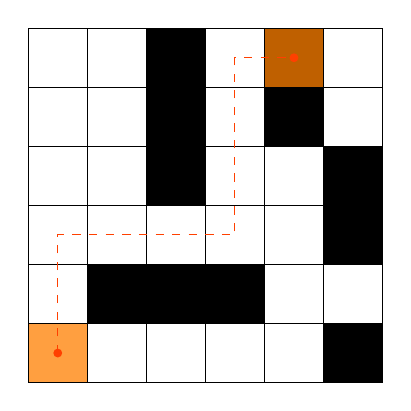
\begin{tikzpicture}[scale=0.75]
			\fill[color=orange!75!white] (0,0) rectangle (1,1);
			\fill (1,1) rectangle (4,2);
			\fill (5,2) rectangle (6,4);
			\fill (5,0) rectangle (6,1);
%			\fill (0,0) -- (1,0) -- (1,1) -- (0,1) -- cycle;
			\fill[color=orange!75!black] (4,5) rectangle (5,6);
			\fill (4,4) rectangle (5,5);
			\fill (2,3) rectangle (3,6);
			\foreach \x in {0,...,5} {
				\foreach \y in {0,...,5} {
					\draw (\x, \y) rectangle (\x+1, \y+1);
				}
			}
			\fill[color=red!50!orange] (0.5, 0.5) circle (0.75mm);
			\fill[color=red!50!orange] (4.5, 5.5) circle (0.75mm);
			\draw[style=dashed, color=red!50!orange] (0.5, 0.5) -- (0.5, 2.5) -- (3.5, 2.5) -- (3.5, 5.5) -- (4.5, 5.5);
		\end{tikzpicture}
		\captionof{figure}{An example with shortest path of length 9}
	\end{minipage}
	\begin{minipage}{0.5\textwidth}
		\centering
		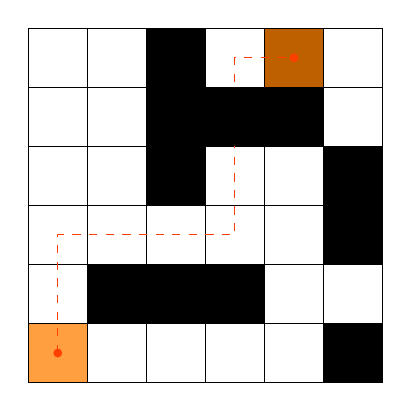
\begin{tikzpicture}[scale=0.75]
			\fill[color=orange!75!white] (0,0) rectangle (1,1);
			\fill (1,1) rectangle (4,2);
			\fill (5,2) rectangle (6,4);
			\fill (5,0) rectangle (6,1);
%			\fill (0,0) -- (1,0) -- (1,1) -- (0,1) -- cycle;
			\fill[color=orange!75!black] (4,5) rectangle (5,6);
			\fill (3,4) rectangle (5,5);
			\fill (2,3) rectangle (3,6);
			\foreach \x in {0,...,5} {
				\foreach \y in {0,...,5} {
					\draw (\x, \y) rectangle (\x+1, \y+1);
				}
			}
			\fill[color=red!50!orange] (0.5, 0.5) circle (0.75mm);
			\fill[color=red!50!orange] (4.5, 5.5) circle (0.75mm);
			\draw[style=dashed, color=red!50!orange] (0.5, 0.5) -- (0.5, 2.5) -- (3.5, 2.5) -- (3.5, 5.5) -- (4.5, 5.5);
			\fill (3,4) rectangle (4,5);
		\end{tikzpicture}
		\captionof{figure}{An example with no solution}
	\end{minipage} \\ \\
	In order to solve this problem, it comes in handy to consider our grid as a graph, where each cell is connected to the ones adjacent to it, excluding the diagonals, since we cannot move diagonally. \\
	\begin{figure}[h]
		\centering
		\begin{tikzpicture}[scale=0.75]
			\draw [<->] (1,0.5) -- (2,0.5);
			\draw [<->] (0,0.5) -- (-1,0.5);
			\draw [<->] (0.5,1) -- (0.5, 2);
			\draw [<->] (0.5,0) -- (0.5, -1);
			\draw [style=dotted] (2.5,-1) -- (2.5,2);
			\draw [style=dotted] (-1.5,-1) -- (-1.5,2);
			\draw [style=dotted] (-1,-1.5) -- (2,-1.5);
			\draw [style=dotted] (-1,2.5) -- (2,2.5);
			\fill[color=white, draw=black] (0,0) rectangle (1,1);
			\fill[color=white, draw=black] (2,0) rectangle (3,1);
			\fill[color=white, draw=black] (-1,0) rectangle (-2,1);
			\fill[color=white, draw=black] (0,-1) rectangle (1,-2);
			\fill[color=white, draw=black] (0,2) rectangle (1,3);
			\draw[style=dashed] (2,2) rectangle (3,3);
			\draw[style=dashed] (-1,2) rectangle (-2,3);
			\draw[style=dashed] (-1,-1) rectangle (-2,-2);
			\draw[style=dashed] (2,-1) rectangle (3,-2);
			

		\end{tikzpicture}
		\caption{An edge between two white vertices represents a possible move}
	\end{figure} \\
	The strategy to solve this exercise will consist in running a \emph{Breath First Search} from our start point, which will traverse all the viable cells (the non-blocked ones) incrementing a counter by one each time we traverse to an adjacent cell, until it eventually I find the exit cell or until there are no more vertices left to be explored, in which case there won't be a solution. \\ \\ 
	This suggest us that our complexity should be in the order of $\mathcal{O}(n+m)$ since that's the complexity of the \emph{BFS} algorithm.
	The most of our complexity, which should instead be $\mathcal{O}(n \cdot m)$, will derive from the fact that we need to parse our standard input into a useful data structure on which we can run our \emph{BFS}. \\ \\
	\newpage
	\lstinputlisting[firstline=3, lastline=10, title=Structure of an individual cell of a grid, firstnumber=1]{ex2.py}
	\lstinputlisting[firstline=23, lastline=60, title=\ , firstnumber=11]{ex2.py}
	\vspace{-0.75cm}
	Implementation of the grid structure, along with class methods, to insert a cell into the grid and to perform a \emph{BFS} from a given cell. The queue used inside the \emph{BFS} is the one from the Python's library. \\ \\ When we happen to find the exit, then we will return the distance that we counted so far, else we will print \say{no} when our queue is empty and there are no other cells to traverse. \\ \\ Our adjacent cells aren't stored anywhere, so from line \verb|33| to \verb|41| we take care to populate the array of adjacents by checking if their coordinate fits within the grid.
	\newpage
	Finally, this is the code that will handle the parsing of the input from string to our meaningful data structure:
	\lstinputlisting[firstline=61, lastline=80, title=\ , firstnumber=53]{ex2.py}
	\vspace{-0.5cm}
	Starting from an empty graph, we will add a cells to it according to the given input, compiling each column for each row of our grid and making our preprocessing time complexity in the order of $\mathcal{O}(n \cdot m)$. \\ \\
	\begin{minipage}{0.2\textwidth}
		Input:
		\begin{lstlisting}
		3 3\end{lstlisting}
	\end{minipage}
	\hfill
	\begin{minipage}{0.8\textwidth}
	~
%		\centering
%		\begin{tikzpicture}
%			\node at (0,0) {\ };
%			\draw[->, thick] (0,1.75) -- (3,1.75)
%				node[pos=0.5, above] {Grid(3,3)};
%		\end{tikzpicture}
%		\hspace{1cm}
%		\begin{tikzpicture}[scale=0.75]
%			\foreach \x in {0,...,2} {
%				\foreach \y in {0,...,2} {
%					\draw (\x,\y) rectangle (\x+1, \y+1);
%					\node at (\x+0.5, \y+0.5) {N};
%				}
%			}
%			\draw [decorate,decoration={brace,amplitude=10pt,mirror,raise=0pt},yshift=0pt, xshift=-2pt] (0, 3) -- (0, 0) node [black,midway,xshift=-0.55cm,yshift=0] {\large n};
%			\draw [decorate,decoration={brace,amplitude=10pt,mirror,raise=0pt},yshift=-2pt] (0, 0) -- (3, 0) node [black,midway,xshift=0,yshift=-0.55cm] {\large m};
%		\end{tikzpicture}
	\end{minipage} \\\\\\
	\begin{minipage}{0.2\textwidth}
		\begin{lstlisting}[firstnumber=2]
		osx\end{lstlisting}
	\end{minipage}
	\hfill
	\begin{minipage}{0.8\textwidth}
		\centering
		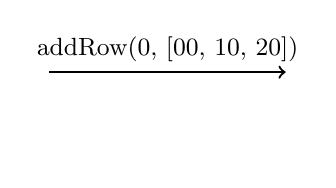
\begin{tikzpicture}
			\node at (0,0) {\ };
			\draw[->, thick] (0,1) -- (3,1)
				node[pos=0.5, above] {\small addRow(0, [00, 10, 20])};
		\end{tikzpicture}
		\hspace{1.8cm}
		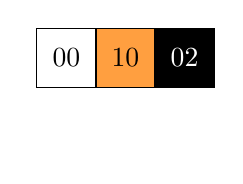
\begin{tikzpicture}[scale=0.75]
			\node at (0, -1) {};
			\fill[color=orange!75!white] (1,0) rectangle (2,1);
			\fill (2,0) rectangle (3,1);
			\foreach \x in {0,...,2} {
				\foreach \y in {0,...,2} {
					\ifthenelse{\y<1}{
						\draw (\x,\y) rectangle (\x+1, \y+1);
						\node at (\x+0.5, \y+0.5) {\x\y};
					}{}	
				}
			}
			\node[white] at (2+0.5, 0+0.5) {02};
		\end{tikzpicture}
	\end{minipage}\\\\\\
	\begin{minipage}{0.2\textwidth}
		\begin{lstlisting}[firstnumber=3]
		xoo\end{lstlisting}
	\end{minipage}
	\hfill
	\begin{minipage}{0.8\textwidth}
		\centering
		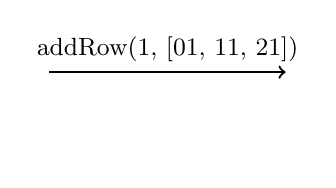
\begin{tikzpicture}
			\node at (0,0) {\ };
			\draw[->, thick] (0,1) -- (3,1)
				node[pos=0.5, above] {\small addRow(1, [01, 11, 21])};
		\end{tikzpicture}
		\hspace{1.8cm}
		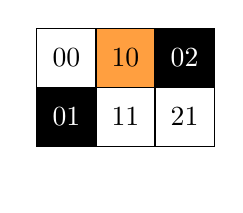
\begin{tikzpicture}[scale=0.75]
			\node at (0,-1.5) {};
			\fill[color=orange!75!white] (1,0) rectangle (2,1);
			\fill (2,0) rectangle (3,1);
			\fill (0,-1) rectangle (1,0);
			\foreach \x in {0,...,2} {
				\foreach \y in {0,...,2} {
					\ifthenelse{\y<2}{
						\draw (\x,\y) rectangle (\x+1, \y-1);
						\node at (\x+0.5, -\y+0.5) {\x\y};
					}{}
					
				}
			}
			\node[white] at (2+0.5, 0+0.5) {02};
			\node[white] at (0+0.5, -1+0.5) {01};
%			\draw [decorate,decoration={brace,amplitude=10pt,mirror,raise=0pt},yshift=0pt, xshift=-2pt] (0, 3) -- (0, 0) node [black,midway,xshift=-0.55cm,yshift=0] {\large n};
%			\draw [decorate,decoration={brace,amplitude=10pt,mirror,raise=0pt},yshift=-2pt] (0, 0) -- (3, 0) node [black,midway,xshift=0,yshift=-0.55cm] {\large m};
		\end{tikzpicture}
	\end{minipage}\\\\\\
	\begin{minipage}{0.2\textwidth}
		\begin{lstlisting}[firstnumber=4]
		eox\end{lstlisting}
	\end{minipage}
	\hfill
	\begin{minipage}{0.8\textwidth}
		\centering
		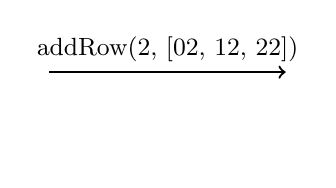
\begin{tikzpicture}
			\node at (0,0) {\ };
			\draw[->, thick] (0,1) -- (3,1)
				node[pos=0.5, above] {\small addRow(2, [02, 12, 22])};
		\end{tikzpicture}
		\hspace{1.8cm}
		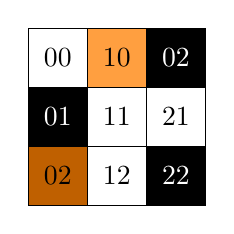
\begin{tikzpicture}[scale=0.75]
			\fill[color=orange!75!white] (1,0) rectangle (2,1);
			\fill (2,0) rectangle (3,1);
			\fill (0,-1) rectangle (1,0);
			\fill[color=orange!75!black] (0,-2) rectangle (1,-1);
			\fill (2,-2) rectangle (3,-1);
			\foreach \x in {0,...,2} {
				\foreach \y in {0,...,2} {
					\draw (\x,-\y) rectangle (\x+1, -\y+1);
					\ifthenelse{\y<3}{
						\node at (\x+0.5, -\y+0.5) {\x\y};
					}{}
					
				}
			}
			\node[white] at (2+0.5, 0+0.5) {02};
			\node[white] at (0+0.5, -1+0.5) {01};
			\node[white] at (2+0.5, -2+0.5) {22};
%			\draw [decorate,decoration={brace,amplitude=10pt,mirror,raise=0pt},yshift=0pt, xshift=-2pt] (0, 3) -- (0, 0) node [black,midway,xshift=-0.55cm,yshift=0] {\large n};
%			\draw [decorate,decoration={brace,amplitude=10pt,mirror,raise=0pt},yshift=-2pt] (0, 0) -- (3, 0) node [black,midway,xshift=0,yshift=-0.55cm] {\large m};
		\end{tikzpicture} 
	\end{minipage} \\ \\ \\ 
	After our input has been preprocessed, the \emph{BFS} will be initialised from our start cell, the reference to which has been saved within our grid data structure. From there, it will traverse all its adjacent cells and the adjacent of those, until it hits the exit cell. The blocked cells have been flagged as \say{already visited} in order for our \emph{BST} to ignore them.
	\newpage
	\begin{figure}[H]
		\centering
		Initially, the BFS will start from the start cell that we had defined in the Grid and start to look for other adjacent cells: \\
		\vspace{0.5cm}
		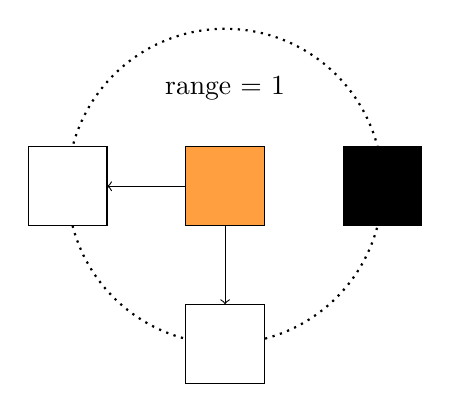
\begin{tikzpicture}
			\draw[style=dotted, thick] (0.5,0.5) circle (2cm);
			\draw[->] (0,0.5) -- (-1, 0.5);
			\draw[->] (0.5,0) -- (0.5, -1);

			\node at (0.5,1.75) {range = 1}; 
			\filldraw[color=orange!75!white, draw=black] (0,0) rectangle (1,1);
			\fill[color=black, draw=black] (2,0) rectangle (3,1);
			\fill[color=white, draw=black] (-1,0) rectangle (-2, 1);
			\fill[color=white, draw=black] (0,-2) rectangle (1,-1);
		\end{tikzpicture} \\
		\vspace{0.5cm}
		We first visit the top left cell but it does not lead anywhere, the top right isn't accessible so we recurse down on the central cell: \\
		\vspace{0.5cm}

		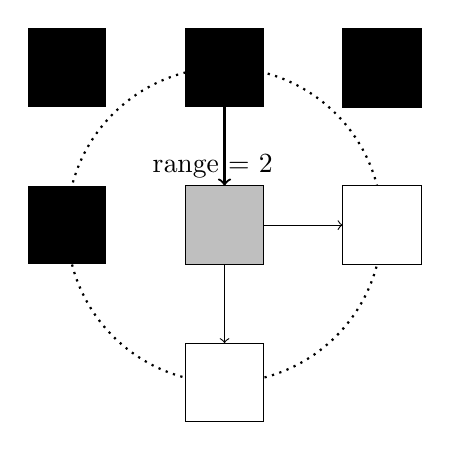
\begin{tikzpicture}
			\draw[style=dotted, thick] (0.5,-1.5) circle (2cm);
			\draw[->, thick] (0.5,0) -- (0.5, -1);
			\draw[->] (0.5,-2) -- (0.5, -3);
			\draw[->] (1,-1.5) -- (2, -1.5);
			\node at (0.35,-0.75) {range = 2}; 
			\fill (0,0) rectangle (1,1);
			\fill[color=black, draw=black] (2,0) rectangle (3,1);
			\fill (-1,0) rectangle (-2, 1);
			\fill[color=gray!50!white, draw=black] (0,-2) rectangle (1,-1);
			\fill (-2,-2) rectangle (-1, -1);
			\fill[color=white, draw=black] (2,-2) rectangle (3, -1);
			\fill[color=white, draw=black] (0,-4) rectangle (1,-3);
		\end{tikzpicture} \\
		The central left cell is blocked, whereas the central right cell does not lead anywhere. Moreover the cell from which we came from can't be revisited, thus we go down the central bottom cell: \\
		\vspace{0.5cm}
		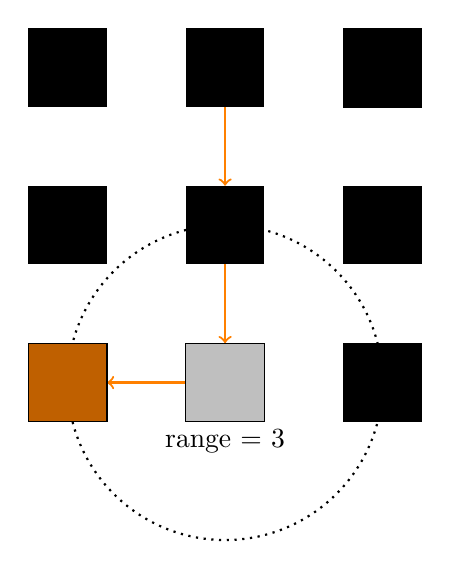
\begin{tikzpicture}
			\draw[style=dotted, thick] (0.5,-3.5) circle (2cm);
			\draw[->, thick, orange] (0.5,0) -- (0.5, -1);
			\draw[->, thick, orange] (0.5,-2) -- (0.5, -3);
			\draw[->, thick, orange] (0, -3.5) -- (-1, -3.5);
			\node at (0.5,-4.25) {range = 3}; 
			\fill (0,0) rectangle (1,1);
			\fill[color=black, draw=black] (2,0) rectangle (3,1);
			\fill (-1,0) rectangle (-2, 1);
			\fill (0,-2) rectangle (1,-1);
			\fill (-2,-2) rectangle (-1, -1);
			\fill (2,-2) rectangle (3, -1);
			\fill[color=gray!50!white, draw=black] (0,-4) rectangle (1,-3);
			\fill (2, -4) rectangle (3,-3);
			\fill[color=orange!75!black, draw=black] (-2, -4) rectangle (-1,-3);
		\end{tikzpicture} \\
		Finally, an exit cell was found next to the current one, thus there is a solution to our maze and the shortest path has been found at range 3!
	\end{figure}
	\newpage
	\subsection{Complexity Analysis}
	The expected time complexity of the program is $\mathcal{O}(n\cdot m)$, since the preprocessing part will take $\mathcal{O}(n \cdot m)$, because we will need to create our adjacency matrix, that is the maze grid that we build from scratch that contains all \verb|None| cells and then inserting all our cells, which is going to take $2(n\cdot m)$ operations. Then our BFS is, according to theory, going to take linear time $n+m$. \\
	This means that our complexity will be $\mathcal{O}(n \cdot m)$.
\end{homeworkExercise}
\\\\
\hspace{5cm}
\section*{Credits}
Both problems were approached alongside \textbf{Cristian Buratti} and \textbf{Riccardo Corrias} the same day the assignment came out. Starting from 11PM we have worked throughout the whole night and managed to solve the assignment by 5AM. As always, we did not share any code among ourselves, however we extensively discussed about the best ways to tackle the problems and we cross checked our programs by running some random inputs and helping in debugging each other's code.
\subsection{Given Help}
I helped \textbf{Alessandra Vicini} in the development of her solution, as she had troubles implementing her own ideas into working code.
\end{document}
